\section{Vista de Implementación}\label{sec:vista-de-implementacion}

La vista de implementación se centra en los componentes en tiempo de ejecución que forman el sistema (ejecutables, bibliotecas y \textit{frameworks}), que son la implementación de los componentes lógicos de la Sección \ref{sec:vista-logica}, y en las dependencias entre ellos.

\subsection{Componentes Ejecutables}

La Tabla \ref{tab:ejecutables} muestra los componentes ejecutables de la solución, la tecnología de cada uno y los subsistemas lógicos que implementan.

\begin{longtable}{|p{3.3cm}|p{5.4cm}|p{6.8cm}|}
    \caption{Componentes ejecutables}\label{tab:ejecutables}\\
    \hline
    \textbf{Componente} & \textbf{Tecnología} & \textbf{Subsistemas que implementa} \\
    \hline
    \endfirsthead
    \hline
    \textbf{Componente} & \textbf{Tecnología} & \textbf{Subsistemas que implementa} \\
    \hline
    \endhead
    \texttt{carga-uy.ear} & Jakarta EE 10 sobre WildFly 41, Java 24. Módulos \texttt{carga-uy-web} (JAX-RS y JSF), \texttt{carga-uy-ejb} (EJB) y \texttt{carga-uy-datos} (JPA con Hibernate). Sesiones con JWT mediante JJWT 0.13; cada request se autentica con un mecanismo de Jakarta Security que valida el JWT, y la autorización se declara con \texttt{@RolesAllowed} en los EJB. & API REST, Backoffice, Servicios de Negocio, Ingesta de Eventos, Adaptador gub.uy y acceso a la Persistencia. \\
    \hline
    Frontend web & React 19 con TypeScript, Tailwind CSS 4 y componentes shadcn/ui, construido con Vite 8. & Frontoffice de Ciudadanos y Frontoffice de Funcionarios. \\
    \hline
    Aplicación móvil & Android (\textit{compileSdk} 37, \textit{minSdk} 26), Kotlin 2.4, Jetpack Compose y Room 2.8 para la persistencia local. & Componente Móvil y su persistencia local. \\
    \hline
    Base de datos & PostgreSQL 17, con el controlador JDBC 42.7.7. & Persistencia. \\
    \hline
    Broker de mensajería & ActiveMQ Artemis embebido en WildFly, con la cola \texttt{queue\_tracking}. & Mensajería. \\
    \hline
    Nodo de tracking simulado & Java 17 con el cliente JMS remoto de WildFly. & Nodo Periférico Tracking. \\
    \hline
\end{longtable}

Todavía no tienen implementación la Generación de Reportes, el Motor de Fiscalización, los adaptadores de la PDI, de notificaciones y de balanzas, el nodo periférico de balanzas y el suplantador de la PDI.

\pendiente{describir los pros y los contras de las tecnologías elegidas y las habilidades necesarias para el proyecto, como pide la plantilla para esta vista.}

\subsection{Dependencias entre Componentes}

La Figura \ref{fig:vista_impl} muestra, con un diagrama de deployment UML \cite{Ambysoft2018}, los artefactos de la Tabla \ref{tab:ejecutables}, el entorno de ejecución en que corre cada uno y las dependencias entre ellos, de acuerdo con el estado actual del repositorio. La distribución prevista para producción se describe en la Sección \ref{sec:vista-de-distribucion}.

\begin{figure}[H]
    \centering
    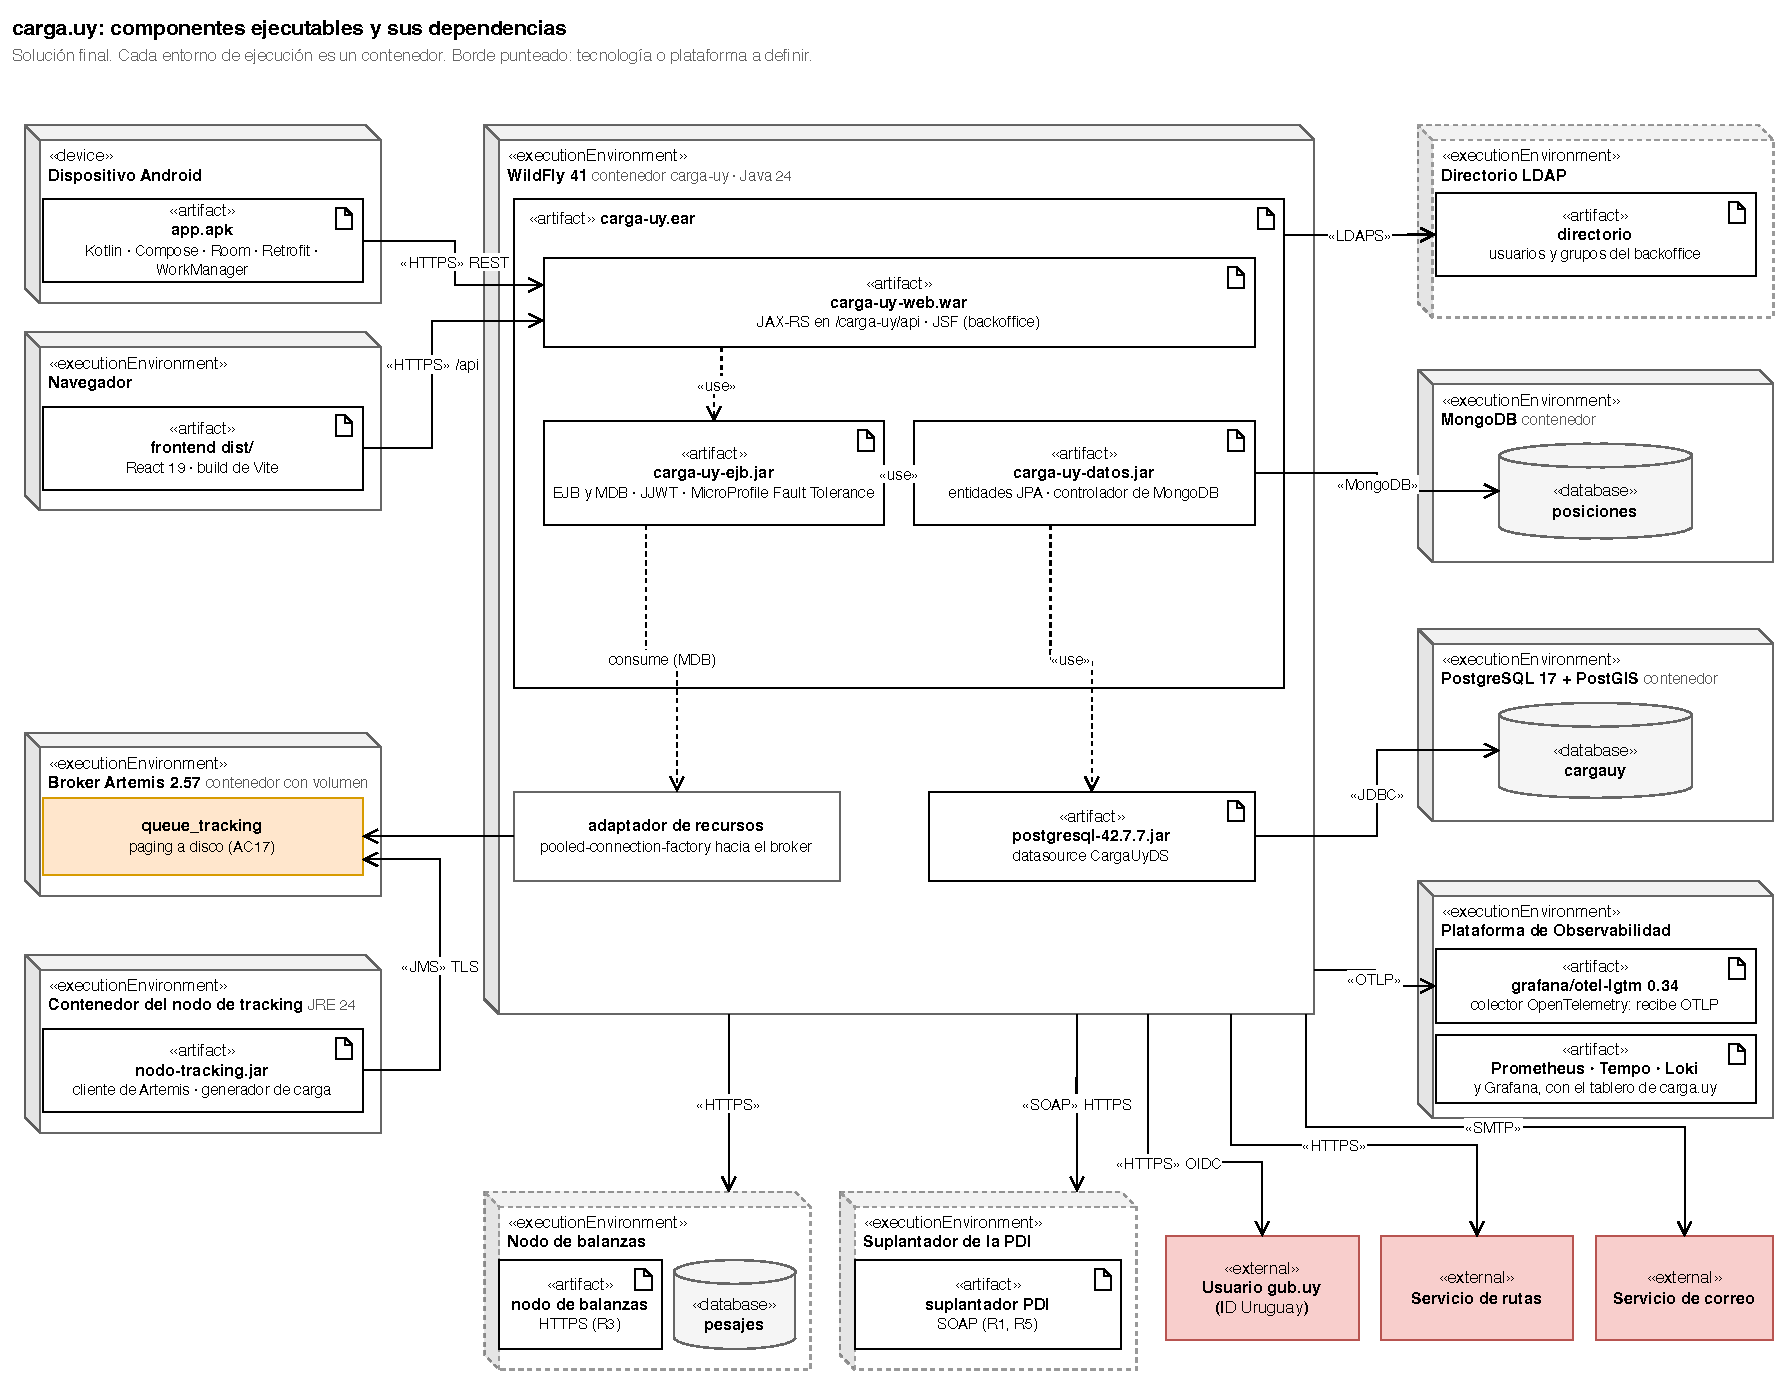
\includegraphics[width=0.9\textwidth]{figures/implementacion.pdf}
    \caption{Vista de Implementación}
    \label{fig:vista_impl}
\end{figure}

\begin{itemize}
    \item Dentro del EAR, \texttt{carga-uy-web} depende de \texttt{carga-uy-ejb}, y este de \texttt{carga-uy-datos}.
    \item El frontend web y la aplicación móvil consumen la API REST del EAR. En desarrollo, el frontend redirige las llamadas a \texttt{/api} hacia el componente central.
    \item El nodo de tracking publica en la cola \texttt{queue\_tracking}, a la que accede como cliente JMS remoto a través del puerto web de WildFly.
    \item El EAR accede a PostgreSQL mediante el \textit{datasource} \texttt{CargaUyDS} y a Usuario gub.uy mediante OpenID Connect.
\end{itemize}

\subsection{Empaquetado}

El componente central se distribuye como una imagen de contenedor construida en dos etapas: la primera compila el proyecto con Maven y la segunda configura WildFly 41 con el controlador de PostgreSQL, el \textit{datasource} y las colas JMS, y despliega el EAR. Un archivo de Docker Compose levanta la base de datos y el componente central. La configuración sensible (credenciales de gub.uy y secreto de los tokens de sesión) se pasa por variables de entorno desde un archivo \texttt{.env} que no se sube al repositorio.

\pendiente{completar R13: el frontend y el nodo de tracking todavía no están contenerizados, así que el entorno completo no se levanta con un único comando. Además, el Dockerfile crea un usuario de WildFly con credenciales escritas en el repositorio (R11).}

\subsection{Integración Continua}

Ante cada modificación, el pipeline del repositorio del grupo en el GitLab de FING debe ejecutar como mínimo la compilación de todos los componentes, las pruebas automatizadas, el análisis estático de calidad del código y la construcción de los artefactos o imágenes de contenedor, y debe estar en estado exitoso al momento de la entrega final (R16, R17).

Hoy el repositorio está en GitHub y tiene un pipeline de GitHub Actions que, en cada \textit{pull request} y en cada cambio en la rama principal, compila el backend, corre las pruebas de \texttt{carga-uy}, \texttt{carga-uy-client} y \texttt{nodo-tracking}, y ejecuta el lint y la construcción del frontend.

\pendiente{migrar el repositorio y el pipeline al GitLab de FING, y agregar el análisis estático de calidad (por ejemplo, SonarQube) y la construcción de las imágenes de contenedor.}
